\section{Wprowadzenie}
\paragraph{}
Ludzie od lat przyzwyczaili się korzystać z elektroniki oraz internetu na standardowych urządzeniach elektronicznych. Na początku lat dziewiędziesiątych do domów zaczęły trafiać komputery stacjonarne. Najpierw z modemami DLS, a następnie już ze stałymi łączami. Na przestrzeni lat korzystanie z ekranu w połączeniu z klawiaturą i myszą stało się dla ludzi naturalne.

Przez ostatnią dekadę na rynku pojawiły się interfejsy dotykowe. Popularność smartfonów, a następnie tabletów spowodowało, że coraz bardziej sporadyznie korzystamy z standardowej fizycznej klawiatury.
Ekrany dotykowe pojawiły się nie tylko na urządzeniach telekomunikacyjnych, lecz także jako moniotory w komputerach pokładowych samochodów oraz instalowane są w zagłówkach w samolotach jako multimedialne centrum rozrywki {\footnote{http://www.komputerswiat.pl/nowosci/wydarzenia/2012/28/boeing-z-androidem-na-pokladzie.aspx}.
\paragraph{}
Przez ostatnie kilka lat narasta trend poszukiwania innych metod dostępu do danych, zwłaszcza multimedialnych. Obecnie wiele przedsiębiorstw prowadzi badania nad nowymi, bardziej naturalnymi interfejsami, które nie wymagałyby użycia standarodwych urządzeń typu klawiatura czy myszka.

Wiele nowych urządzeń próbuje implementować sterowanie intefejsem użytkownika za pomocą gestów (np. Microsoft Kinect\footnote{http://www.xbox.com/pl-PL/xbox-one/accessories/kinect-for-xbox-one}), czy też za pomocą myśli (np. Emotiv{\footnote{http://emotiv.com}). Na rynku widać duże zainteresowanie nową formą kontroli urządzeniami, zwłaszcza tymi bardziej naturalnymi dla człowieka.

\paragraph{}
Na przestrzeni lat interfejsy urządzeń elektronicznych ewoluowały pierwotnie z aplikacji sterowanych za pomocą wiersza polecań poprzez programy z graficznym interfejsem użytkownika (Graphic Uuser Interface), aż do obecnie coraz bardziej popularnej i rozwijanej grupy interfejsów ,,naturalnych'' (Natural User Interface).
\begin{center}
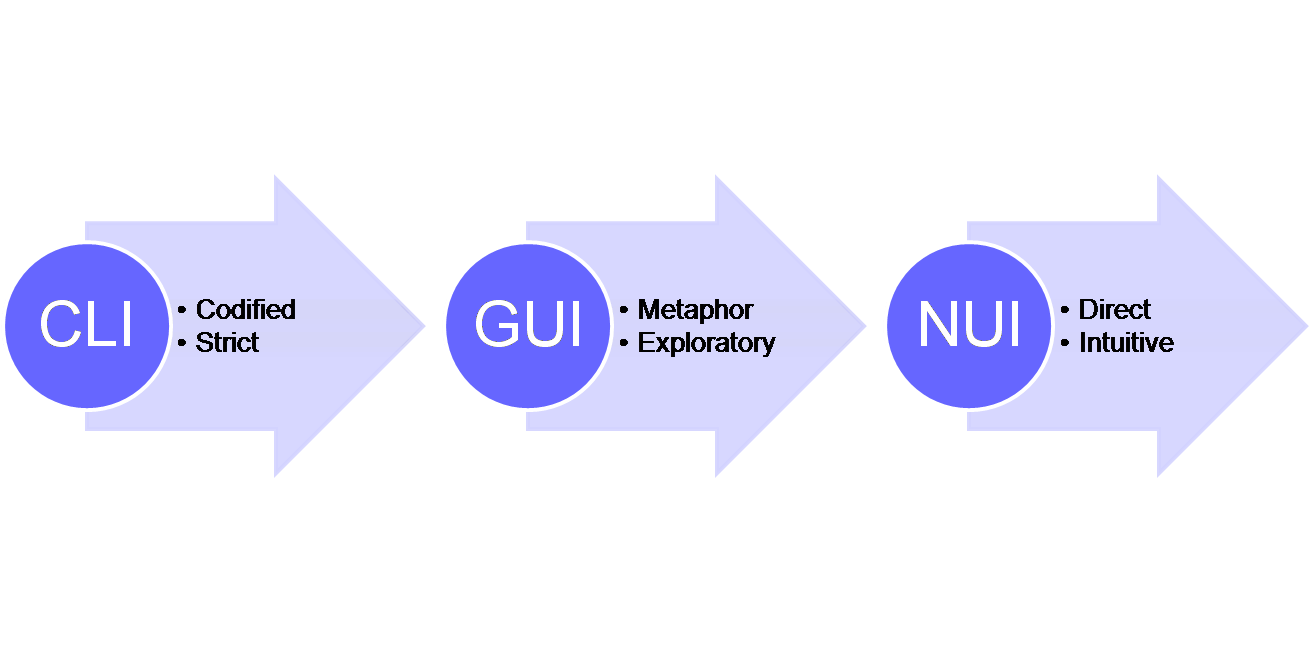
\includegraphics[width=0.9\textwidth]{images/nui.png}
\captionof{figure}{
Ewolucja interfejsów użytkownika
}
\small {źródło: https://en.wikipedia.org/wiki/Natural\_user\_interface }
\end{center}

\paragraph{}
W branży filmowej oraz gier wideo narasta trend używania nowych technologii do rozszerzania doznań jakie otrzymuje odbiorca.
W kinach odbywają są coraz częściej projekcje filmów stworzonych w technologii trójwymiarowej. Natomiast w ostatnim czasie pojawią się sale kinowe pozwaljące  na projecję filmów trójwymiarowych wraz z dodatkowymi elementami takimi jak: drganie foteli, wiatr, dym, woda \footnote{http://cinema-city.pl/4dx-info}. Jednakże w obecnej chwili taki format rozrywki jest dość drogi, gdyż wymaga specjalnie przygotowanej sali kinowej oraz okularów, które pozwalają tworzyć iluzję przestrzenną. 

\subsection{Rozszerzona rzeczywistość}
\paragraph{}
Coraz bardziej popularne staje się pojęcie rozszerzonej rzeczywistości (ang. augmented reality). Jest to zbiór różnych technologii pozwalającej łączyć świat rzeczywisty z wirtualnym. Jest to jezcze mało popularny sposób interakcji, lecz w ostatnim dziesięcioleciu rozwój (zarówno urządzeń jak i specjalistycznego oprogramowania) jest bardzo dynamiczny.
\paragraph{}
Pierwsze próby w tej dziedzinie odbywały się jeszcze w latach sześćdziesiątych amerykański naukowiec oraz artysta Myron Krueger  prowadził badania nad wirtualną oraz rozszerzoną rzeczywistością.

dopisac dalej..

\paragraph{}
Natural Machines, Meta2, Wonderbook
\begin{center}
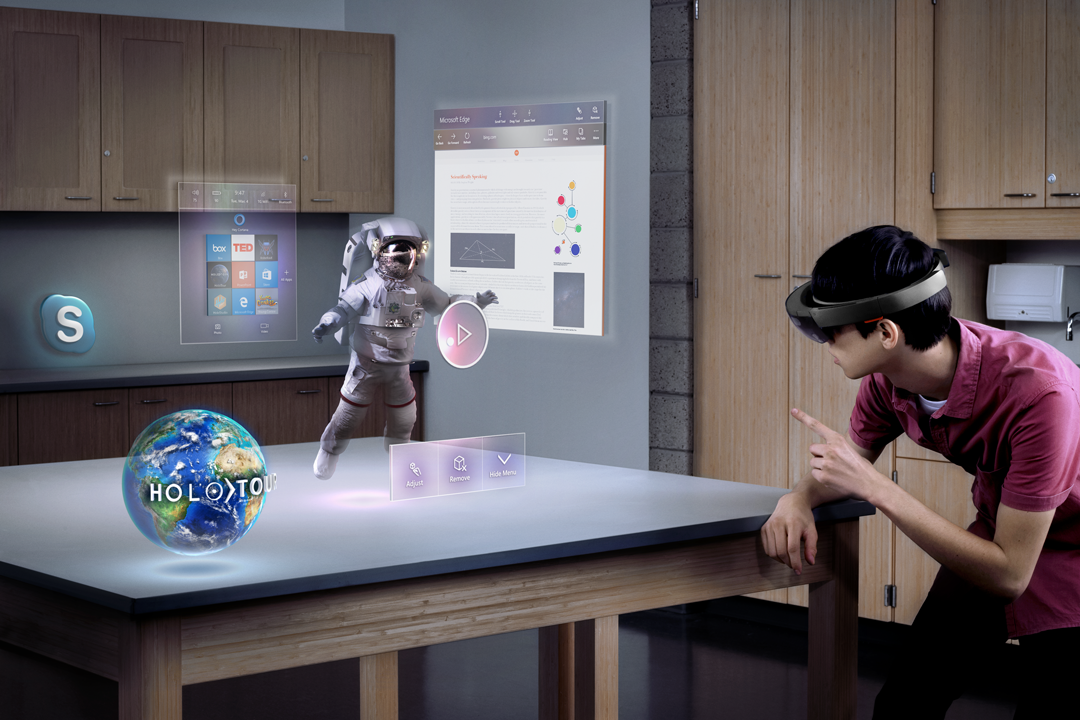
\includegraphics[width=0.9\textwidth]{images/hololens.png}
\captionof{figure}{
Wizualizacja Microsoft HoloLens
}
\small {źródło: https://www.microsoft.com/microsoft-hololens/en-us/why-hololens }
\end{center}